\subsection{Funksjoner}
\begin{frame}{Funksjoner}
    Funksjoner kjenner vi fra INF100 i fjor. Nå skal vi formalisere dem litt mer.\\
    \begin{columns}
        \begin{column}{0.5\textwidth}
            Fra nå av ser vi på datatyper som sett:
            \begin{itemize}
                \item $int := \mathbb{Z}$
                \item $str := \{$ "a", "b", "c", "aa", "ab", ... $\}$
            \end{itemize}
            Domenet til en funksjon er inputsettet.\\
            Kodomenet til en funksjon er outputsettet.
        \end{column}
        \pause
        \begin{column}{0.5\textwidth}
            \begin{figure}
               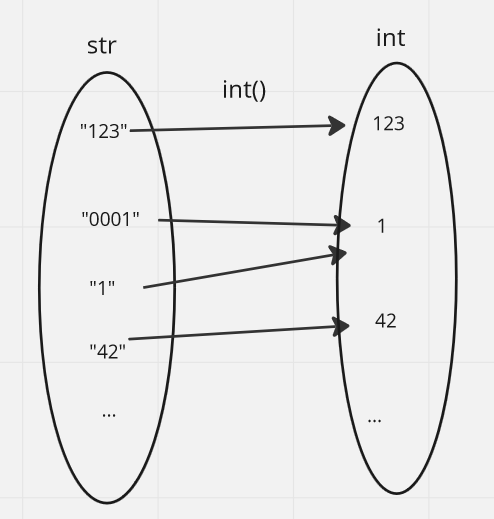
\includegraphics[scale = 0.4]{images/int.png} 
               \caption{$int : str \rightarrow int$}
            \end{figure}   
        \end{column}
    \end{columns}
\end{frame}

\begin{frame}{Funksjonskomposisjon}
    \begin{columns}
    \begin{column}{0.38\textwidth}
Gitt to funksjoner:
    \begin{itemize}
        \item $f : A \rightarrow B$
        \item $g : B \rightarrow C$
    \end{itemize}
Kan vi definere en unik tredje funksjon: \\
    $g \circ f : A \rightarrow C$\\
    $g \circ f := g(f(x))$\\
    \pause
    \end{column}
    \begin{column}{0.55\textwidth}
        \centering
        La $f(x) := x+1$, og $g(x) := x/2$.\\
        Da er $g \circ f = g(f(x)) = (x+1)/2$.\\
        \begin{figure}
            \centering
            \subfloat{{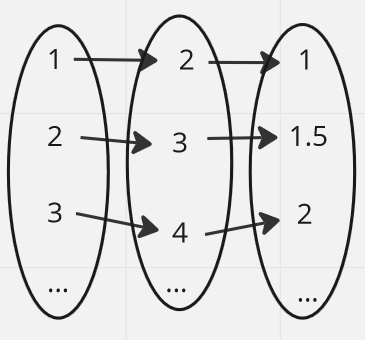
\includegraphics[width=2.8cm]{images/f, g.png} }}%
            \qquad
            \subfloat{{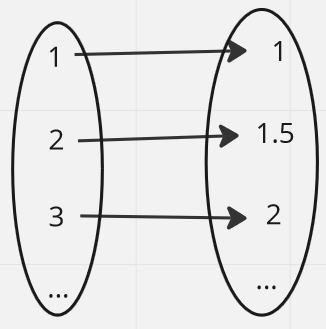
\includegraphics[width=2.8cm]{images/g o f.png} }}%
            \label{fig:g o f}
        \end{figure}
    \end{column}
    \end{columns}
    \pause
    Obs! Rekkefølgen er uintuitiv. $f$ skjer før $g$. Dere kan lese det som $g$ 'anvendt på' $f$.
\end{frame}

\begin{frame}{Injektivitet}
En funksjon $f : A \rightarrow B$ er \emph{injektiv} hvis $\forall a_1, a_2 \in A : [f(a_1) = f(a_2) \rightarrow a_1 = a_2]$.\\
Med andre ord: alle inputs gir et unikt output og alle piler peker på forskjellige ting.
    \begin{figure}%
        \centering
        \subfloat[\centering Ikke injektiv]{{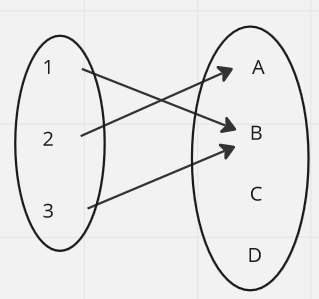
\includegraphics[width=3.2cm]{images/Ikke inj.png} }}%
        \qquad
        \subfloat[\centering Injektiv]{{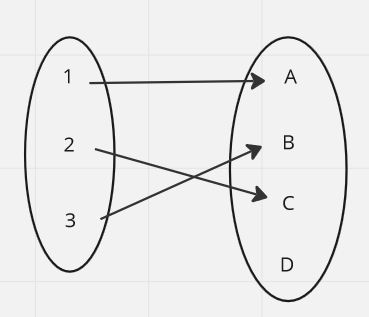
\includegraphics[width=3.2cm]{images/Inj.png} }}%
        \qquad
        \subfloat[\centering Ikke injektiv]{{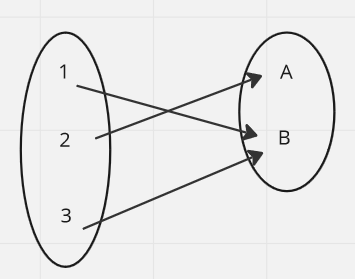
\includegraphics[width=3.2cm]{images/Heller ikke inj.png} }}%
        \label{fig:inj}%
    \end{figure}
    \pause
    Observer at det finnes en injeksjon hvos og bare hvis $|B| \geq |A|$.
\end{frame}

\begin{frame}{Surjektivitet}
En funksjon $f : A \rightarrow B$ er \emph{surjektiv} hvis $\forall b \in B$ $\exists a \in A: [f(a) = b]$.\\
Med andre ord: hele kodomenet/outputsettet blir brukt og alt i $B$ har minst én pil som peker på seg.
    \begin{figure}%
        \centering
        \subfloat[\centering Ikke surjektiv]{{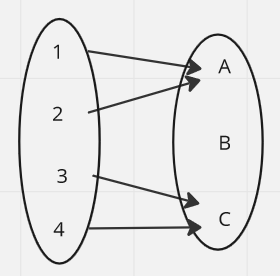
\includegraphics[width=3.2cm]{images/Ikke surjektiv.png} }}%
        \qquad
        \subfloat[\centering Surjektiv]{{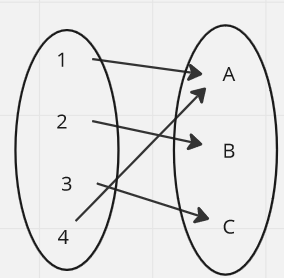
\includegraphics[width=3.2cm]{images/Surjektiv.png} }}%
        \qquad
        \subfloat[\centering Ikke surjektiv]{{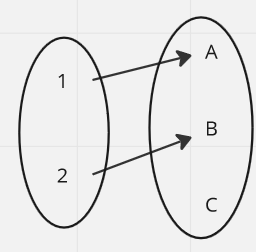
\includegraphics[width=3.2cm]{images/Aldri surjektiv.png} }}%
        \label{fig:sur}
    \end{figure}
    \pause
    Observer at det finnes en surjeksjon hvis og bare hvis $|A| \geq |B|$.
\end{frame}

\begin{frame}{Bijektivitet}
En funksjon $f : A \rightarrow B$ er \emph{Bijektiv} om den er både injektiv og surjektiv.\\
    \pause
    Da finnes det en unik invers funksjon $f^{-1} : B \rightarrow A$ slik at $f^{-1} \circ f = id_A$ og $f \circ f^{-1} = id_B$, dvs at $\forall a \in A : [a = f^{-1}(f(a))]$ og $\forall b \in B : [b = f(f^{-1}(b))]$.
    \pause
\begin{figure}
        \centering
        \subfloat[\centering Surjektiv, ikke injektiv]{{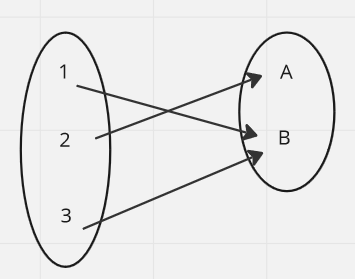
\includegraphics[width=2.4cm]{images/Heller ikke inj.png} }}%
        \qquad
        \subfloat[\centering Injektiv, ikke surjektiv]{{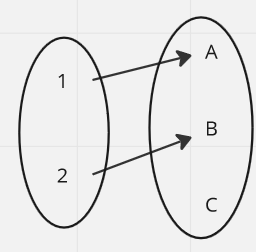
\includegraphics[width=2.4cm]{images/Aldri surjektiv.png} }}%
        \qquad
        \subfloat[\centering Bijektiv]{{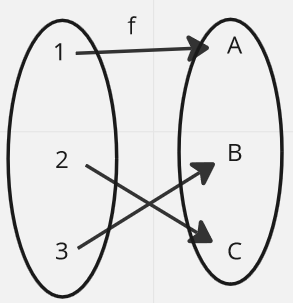
\includegraphics[width=2.4cm]{images/Bijektiv f.png} }}
        \qquad
        \subfloat[\centering Inverset $f^{-1}$]{{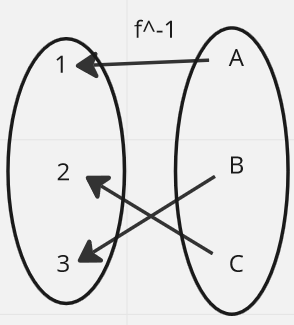
\includegraphics[width=2.4cm]{images/Invers f.png} }}%
        \label{fig:bij}
    \end{figure}

    \pause
    Observer at det finnes en bijeksjon hvis og bare hvis $|A| = |B|$.
\end{frame}

\begin{frame}{Tavleoppgaver om injektivitet, surjektivitet, bijektivitet}
    \begin{itemize}
        \item Injektiv:  $\forall a_1, a_2 : [f(a_1) = f(a_2) \rightarrow a_1 = a_2]$.\\
        \item Surjektiv: $\forall b \in B$  $\exists a \in A : [f(a) = b]$.\\
        \item Bijektiv: begge de over \\
    \end{itemize}
    \pause
    \begin{block}{Avgjør om de følgende funksjonene er injektive, surjektive, eller bijektive:}
        $even : \mathbb{Z} \rightarrow $ Bool, $even(x) := x$ mod $2 = 0$\\
        $f : \mathbb{R} \rightarrow \mathbb{R}$, $g(x) := e^x$\\
        $g : \mathbb{R} \rightarrow \mathbb{R}^+$, $g(x) := e^x$\\
        $h : \mathbb{R} \rightarrow \mathbb{R}$, $h(x) := 2x + 1$\\
        $k : \mathbb{Q} \rightarrow \mathbb{N}$, $k(x) := 1$\\
    \end{block}
    \pause
    Noen kaller surjektive funksjoner for 'onto' på engelsk. Mens 'one-to-one', eller 1-1, kan bety enten bijektiv eller injektiv avhengig av hvem som sier det.
\end{frame}